

When performing software tasks in large and complex software systems, software developers typically consult several different kinds of documents, or artifacts, that assist them in their work~\cite{Starke2009, Meyer2017}. For example, 
when incorporating a new software library needed for a new feature, a developer might consult official application programming interface (API) documents for the library~\cite{robillard2011field, umarji2008archetypal} or 
 question-and-answer developer forums~\cite{parnin2012, silva2019}.



Many of the artifacts that developers consult
contain unstructured text; for the purposes of this thesis, we refer to artifacts with unstructured text as natural language artifacts.  
To utilize information in  natural language artifacts, a developer must read the text to find the information that is relevant to the task being performed~\cite{Bavota2016}.
However, 
the sheer amount of information in these natural language artifacts may prevent a developer from comprehensively assessing what is useful to their task~\cite{Murphy2005}.
Within just one kind of artifact, API
documentation, studies have shown that it can take 15 minutes or more
of a developer's highly constrained time to identify 
information needed to perform certain task~\cite{endrikat2014, Meyer2017}. 
Considering that a developer must typically
consult multiple kinds of documents
when performing a task, the time investment to find the needed information can be significant
and a developer that fails to locate all, or most, of the information needed
will have an incomplete or incorrect basis from which to perform a software task.



Finding information that assists a developer to complete a task can be a time-consuming
 and cognitively frustrating process~\cite{Begel2008,
 robillard2011field}. Therefore, we posit the need for approaches that assist developers in locating information in the different natural language artifacts sought  as part of a software task.

 
 



 \section{Scenario}
 \label{cp1:example}
 
 
 
 To illustrate challenges in locating information useful for a task, let us consider an  Android mail client application\footnote{\url{https://github.com/k9mail/k-9}}.
 Figure~\ref{fig:android-notifications-task} shows a task---in the form of a GitHub issue\footnote{\url{https://github.com/k9mail/k-9/issues/1741}}---that indicates that 
 app notifications 
 are not working as expected in Android 7.0. 
 
 \medskip
 \begin{figure}[h!]
     \centering
     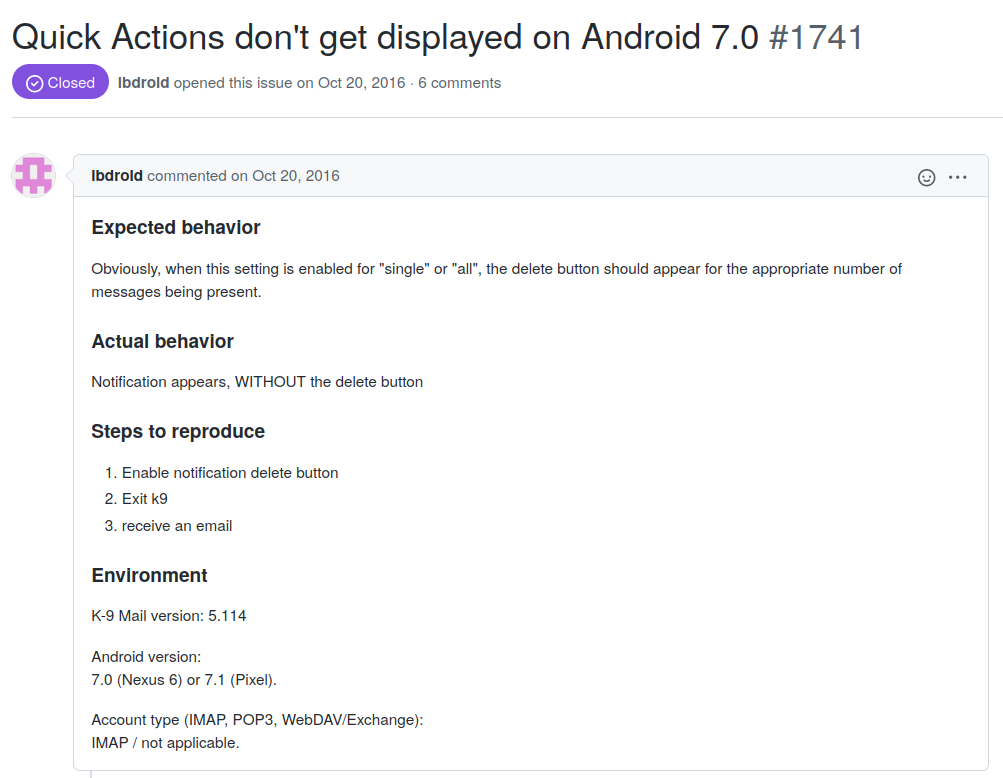
\includegraphics[width=\dimexpr\linewidth-4\fboxsep-2\fboxrule]{cp1/android-quick-actions}
     \caption{k-9 mail GitHub issue \#1741 indicating that quick actions don't get displayed on Android 7.0}
     \label{fig:android-notifications-task}
 \end{figure}
 
 
 \medskip
 A developer assigned to this issue might not be familiar with how Android notifications work and thus, they will likely need additional knowledge to understand and resolve this task~\cite{ko2007, Li2013, sillito2006}. 
 Often, this knowledge can be acquired from a developer's peers~\cite{singer2011}. 
 However, the fragmented and distributed nature of software development  
 may prevent the developer from accessing their peers~\cite{ko2007},
 instead they seek online web resources for information 
 that may assist them in completing the task-at-hand~\cite{Xia2017, rao2020}.
 
 
 
 
 
 \begin{figure}
     \centering
     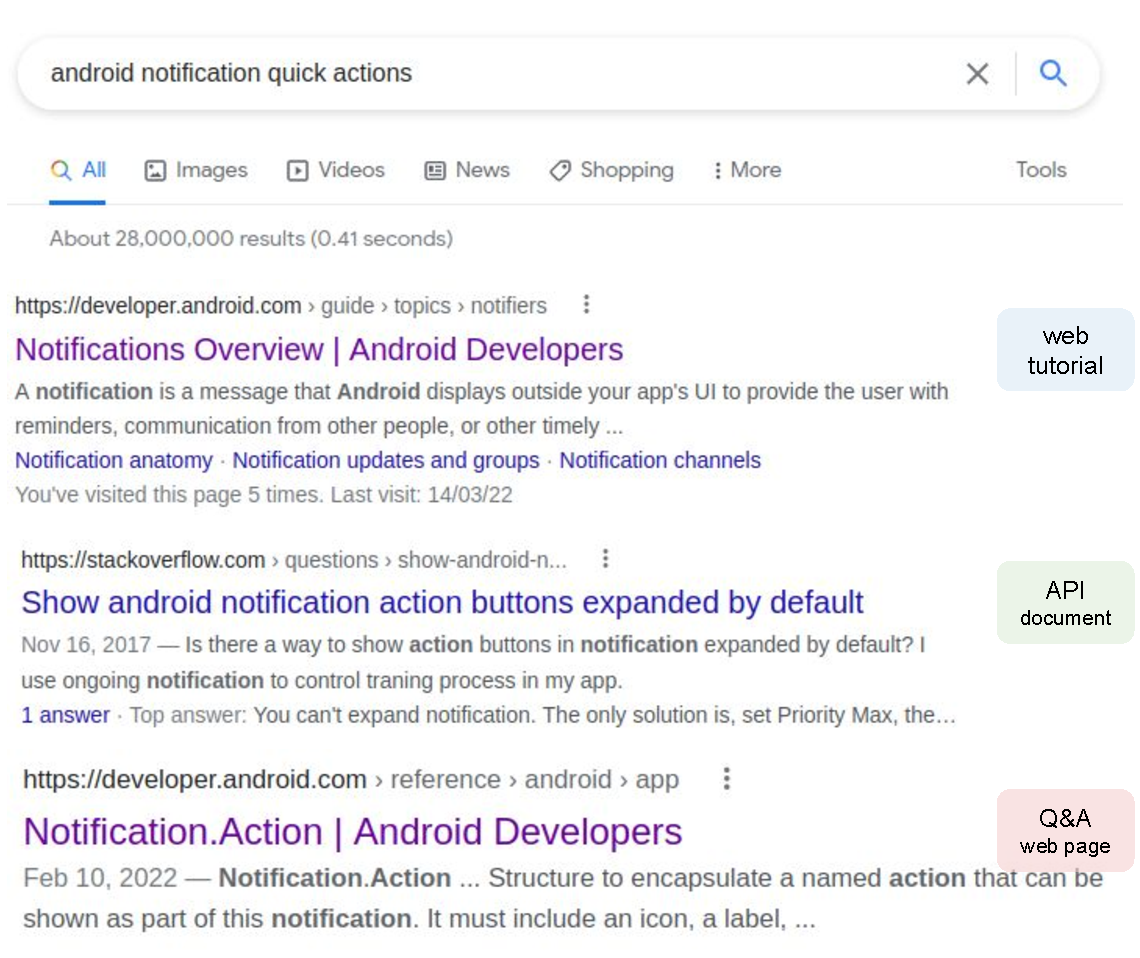
\includegraphics[width=.95\textwidth]{cp1/search-results.pdf}
     \caption{Search results showing artifacts of potential interest to the Android quick actions issue}
     \label{fig:android-search-results}
 \end{figure}
 
 
 
A common way to find software artifacts
pertinent to the developer's task
is through a web search engine~\cite{Brandt2009a, Li2013}.
Figure~\ref{fig:android-search-results}
shows the artifacts resulting from a developer's search 
about android notifications for the task in Figure~\ref{fig:android-notifications-task}.
Each artifact can be assigned a type. For instance,
the artifacts returned represent web tutorials, API documents and question-and-answer
artifacts, each of which can be considered a different type,
where each type of artifact has different associated challenges for locating 
information useful to a task within them.



% https://tex.stackexchange.com/questions/339026/how-to-make-the-text-float-around-figures-in-landscape-mode
% https://tex.stackexchange.com/questions/468393/including-large-images-in-landscape-formatting


\afterpage{
\begin{landscape}
\begin{figure}
    \centering
    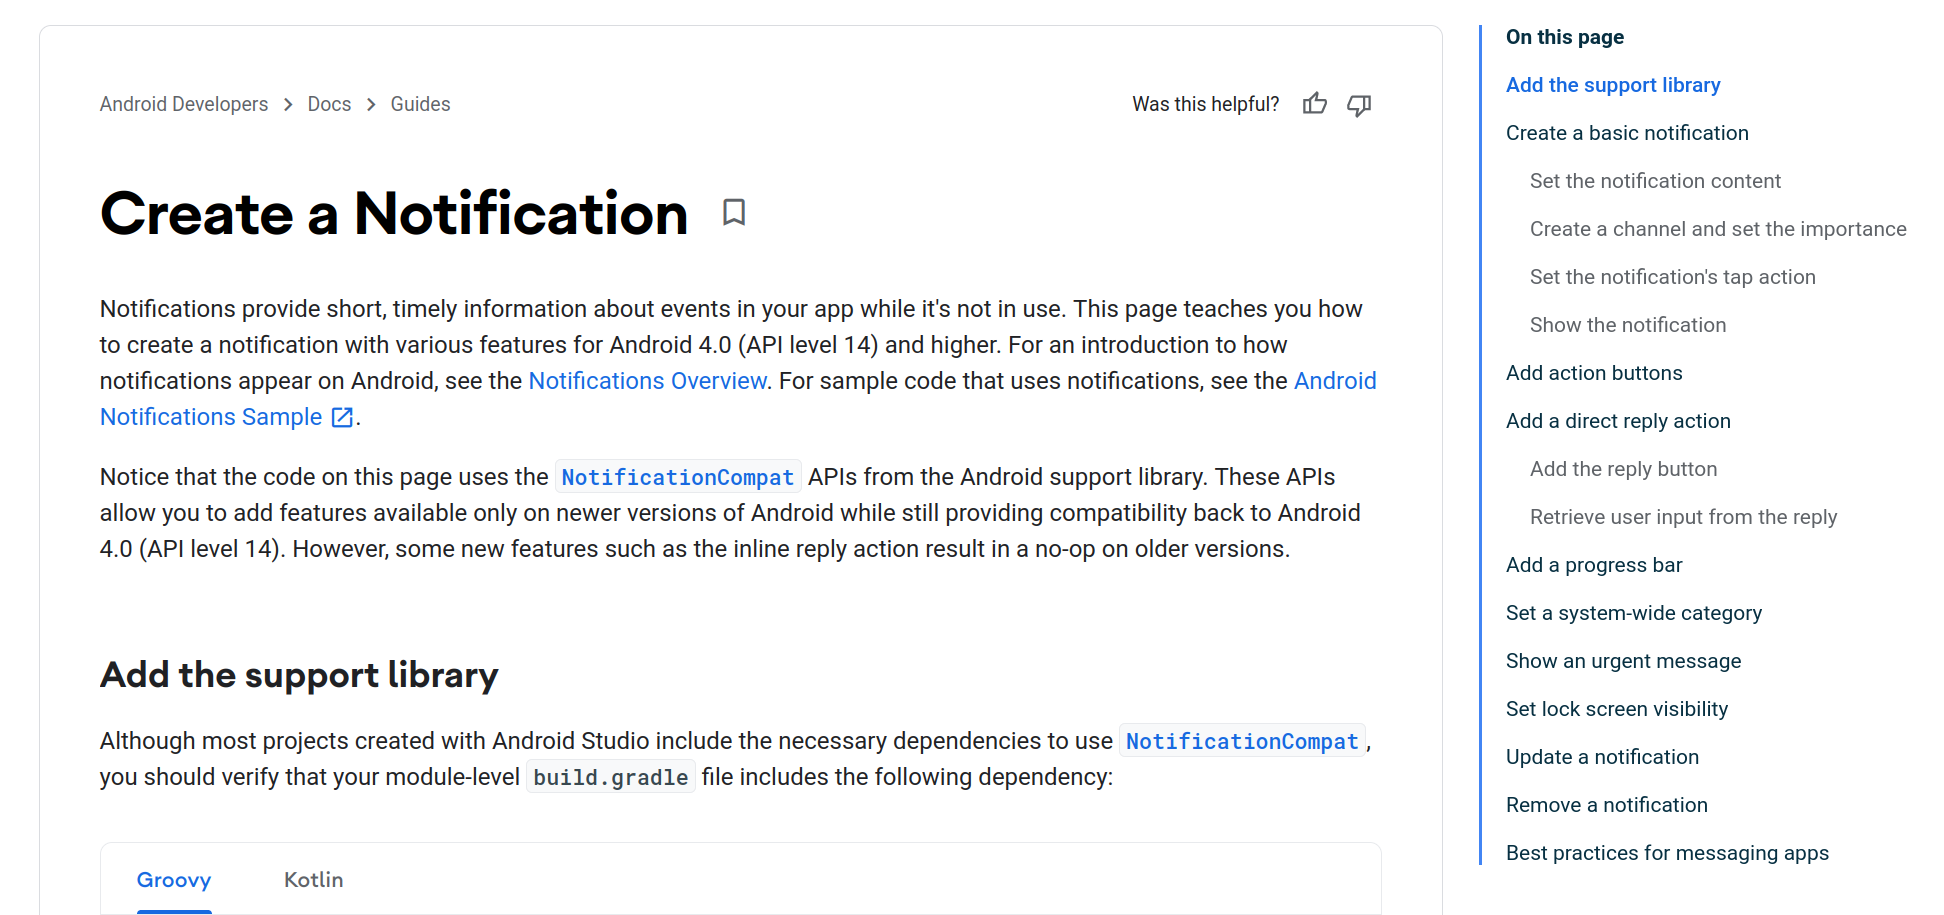
\includegraphics[width=\dimexpr\linewidth-4\fboxsep-2\fboxrule]{cp1/create-notification.png}
    \caption{Snapshot of the official Android notifications tutorial  with highlights relevant to the GitHub issue \#1741}
    \label{fig:tutorial-create-notification}
\end{figure}
\end{landscape}
}

The first artifact in Figure~\ref{fig:android-search-results}
is a 
 web tutorial, a document intended primarily to teach users how to use 
a technology~\cite{arya2020} through a series of structured topics 
that progressively explain concepts about the technology~\cite{Jiang2016b, Jiang2017}. 
Figure~\ref{fig:tutorial-create-notification} 
shows a portion of this artifact's content. 
The Android tutorial contains  approximately 200 sentences
and, on the page's right-hand side, we find that 
it
has nine sections, each with sub-sections of their own. 
Reading all sections of this document could potentially 
take 10 minutes or more\footnote{Using a standard reading metric of 200 words per minute~\cite{Just1980}.} of a developer's time.
To save time, a developer would likely try to find the sections of the document
most closely related to their task~\cite{Li2013}.
For example, using a web browser's search to find content that mentions the `\textit{actions}' keyword, 
a developer would find eight different matches spread across four different sections.
Not all of these matches will be relevant, requiring the developer to peruse each
match and assess relevance. 
For instance, the `\textit{Notification actions}'
 (under focus in the figure), 
explains 
notifications for both Android version 7.0 and 12.0, 
 but given that the developer's task is related to the former version,
only the text highlighted (in orange)
might be of relevance to the task we presented in Figure~\ref{fig:android-notifications-task}.






An \acs{API} 
contains software elements (e.g., classes and methods) that other developers 
are   expected to use for a certain purpose~\cite{monperrus2012}. Instructions about an API usage are typically available in the API's reference documentation.
Figure~\ref{fig:api-notification-action} shows part of the reference documentation for one of the classes of the Android API, namely `\textit{Notification.Action}'. 
In the right-hand side of the figure, we find common 
information in this type of artifact, including a brief summary,
constants and fields available, the class's constructor, and 
each of the functions or methods that this particular class provides,  
for a total of 35 distinct elements.
To find the portions of the text relevant to
their task,
a developer unfamiliar with this document would 
face challenges similar to the ones already  described in the web tutorial. Additionally, 
we note that complex APIs, 
such as the ones exposed by the Android operating system, require combining several classes
and method calls~\cite{robillard2011field} to properly perform some instruction,
which would mean inspecting at least three other classes 
with equally complex documentation
to find all the text explaining the API elements used in the quick actions menu\footnote{\url{https://github.com/k9mail/k-9/pull/1755/files}}.





\begin{figure}
    \centering
    \makebox[\textwidth][c]{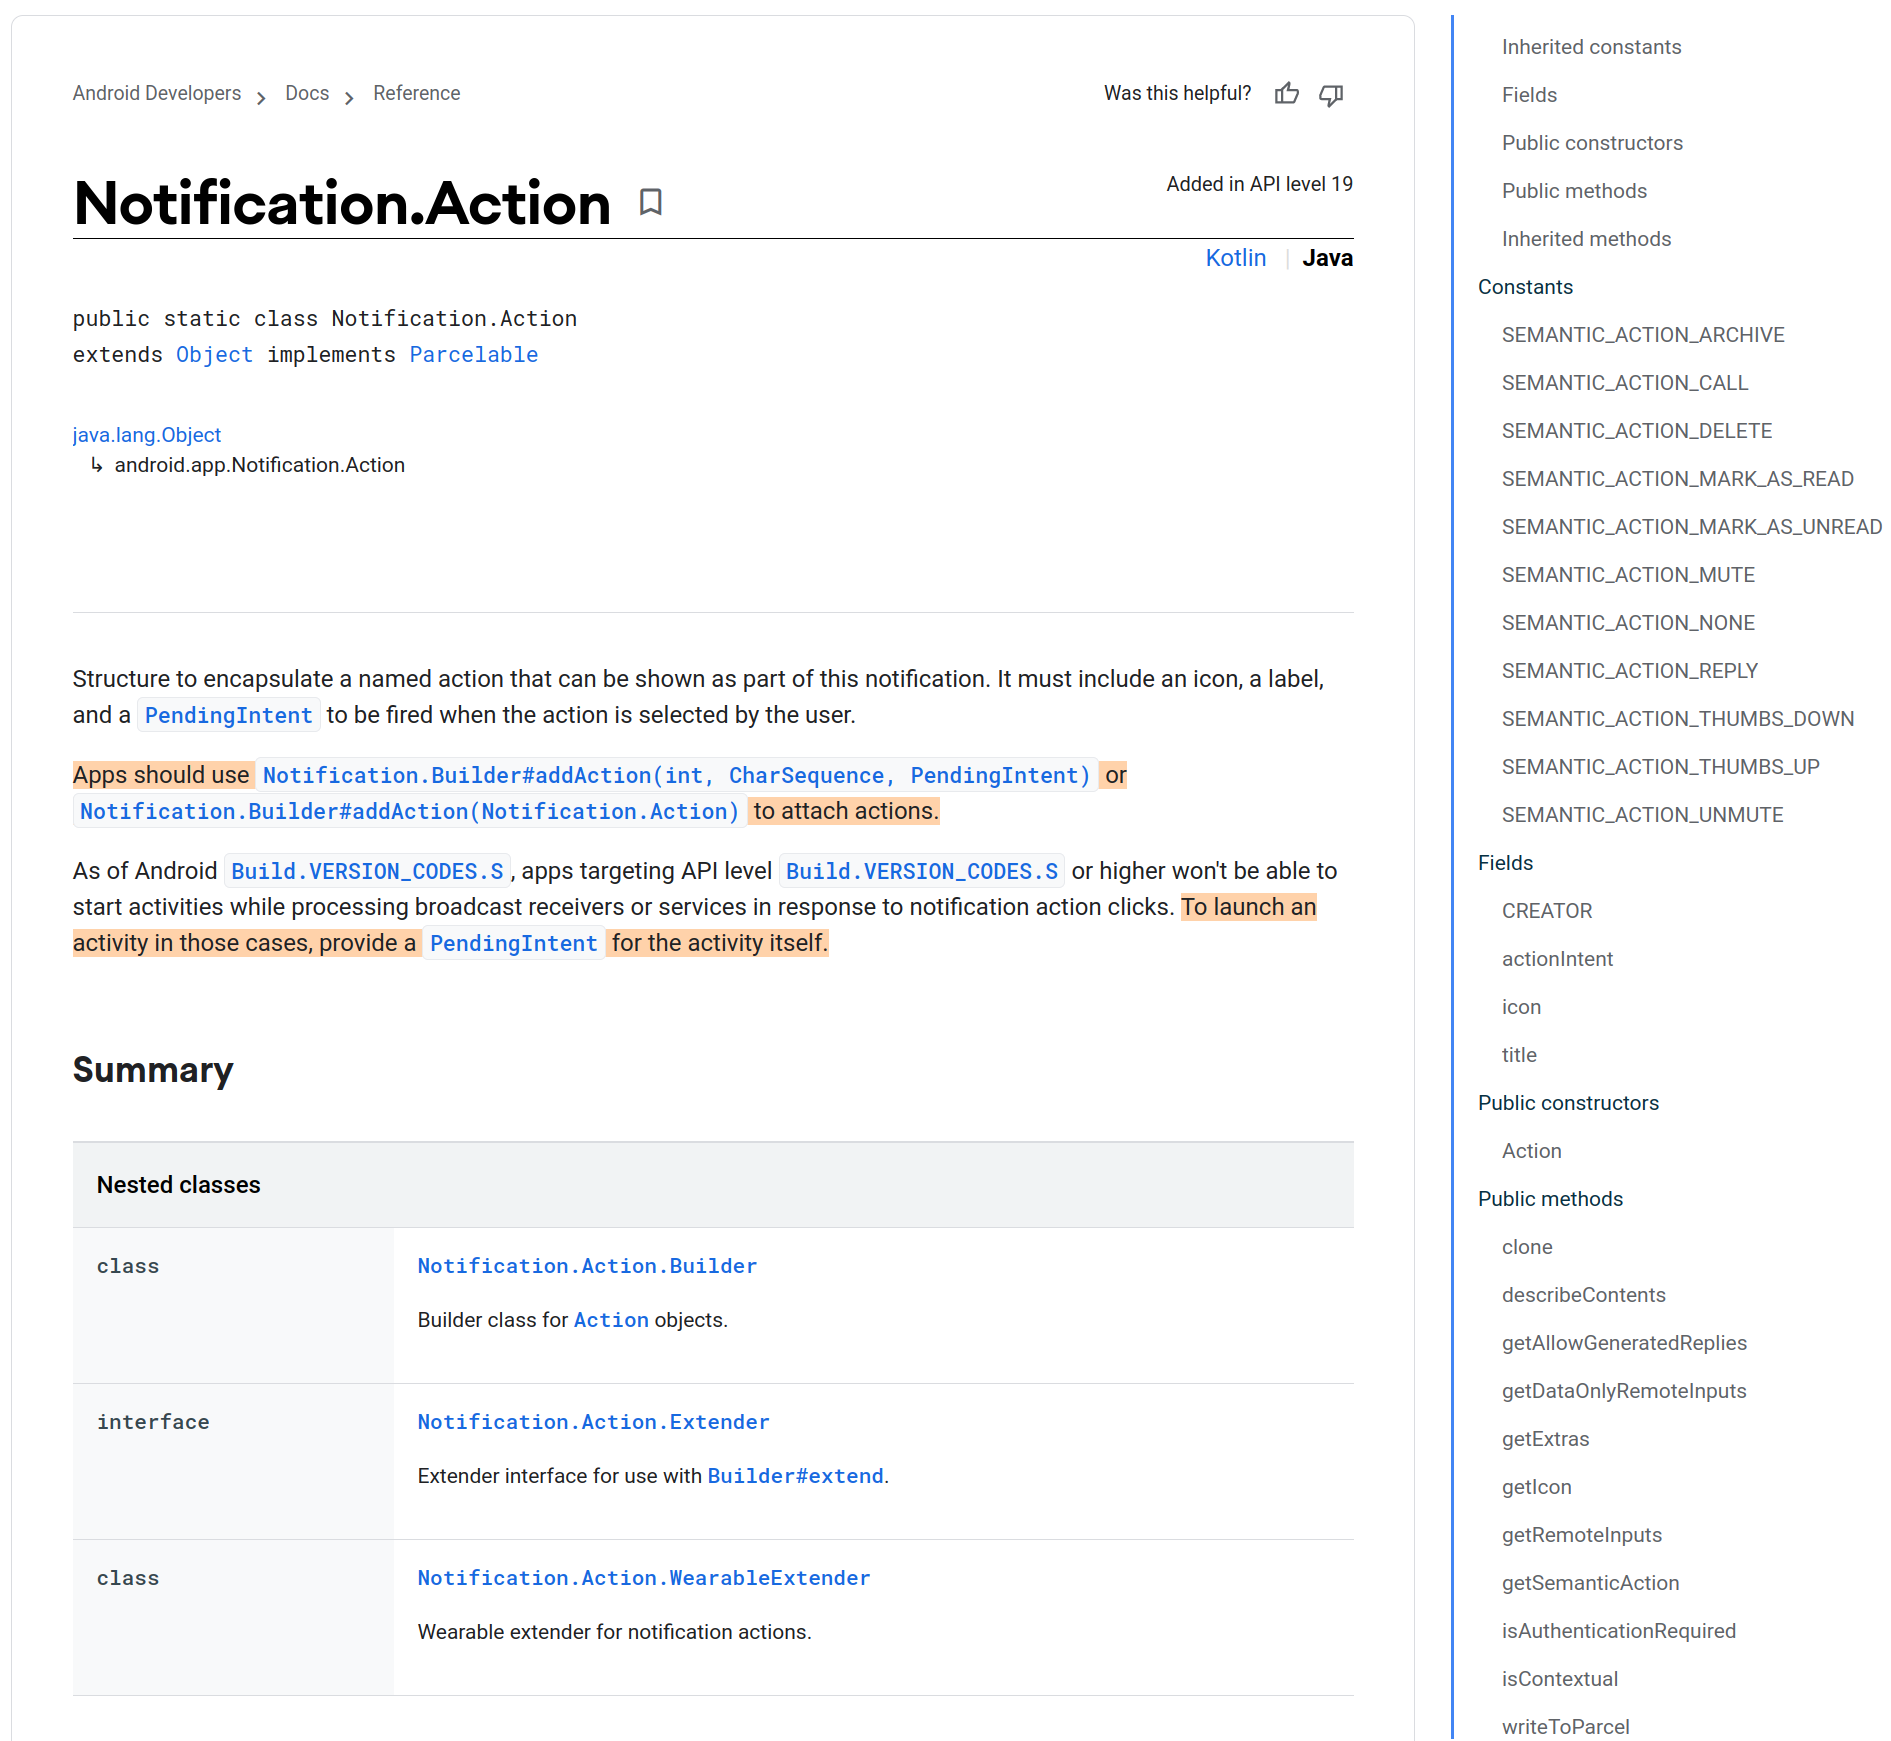
\includegraphics[width=1.2\textwidth]{cp1/notification-action.png}}
    \caption{Snapshot of the Android Notification.Action API reference documentation with highlights relevant to the GitHub issue \#1741}
    \label{fig:api-notification-action}
\end{figure}





\begin{figure}
    \centering
    \makebox[\textwidth][c]{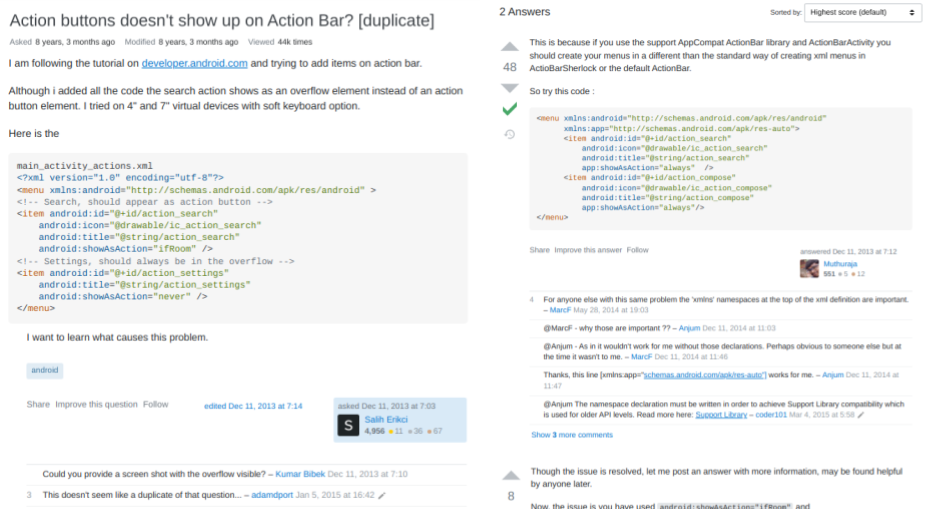
\includegraphics[width=1.2\textwidth]{cp1/stackoverflow-notifications.png}}
    \caption{Snapshot of a Stack Overflow question about Android notifications  with highlights relevant to the GitHub issue \#1741}
    \label{fig:qa-notification-icon}
\end{figure}


The third artifact resulting from the developer's search 
about android notifications 
is a post in a \acf{qa} web platform, Stack Overflow\footnote{\url{https://stackoverflow.com/}}.
Figure~\ref{fig:qa-notification-icon} shows an example of the information found in this type of artifact.
A question usually contains both text and code snippets
and it includes a set of tags  about the
problem's programming language or technology~\cite{Treude2011a}. 
Each answer contains similar content and 
the counter that appears on left of a question and of each answer
represents how many other users found them helpful (or not).
The user who asked the question can also accept an answer (green check mark)
if it correctly solved their problem.
We also find a list of similar or related questions 
at the right portion of the page. 
This more structured format often assists a developer 
in navigating through the content in this type of artifact~\cite{nadi2020}, for example, a developer could read the problem and 
then the accepted answer to quickly find information that might be helpful 
to their task. Nonetheless, a series of factors make finding useful information challenging. 
For instance, only half of the Android questions on Stack Overflow
have an accepted answer~\cite{parnin2012} 
and millions of questions have more than one answer~\cite{nadi2020}.
Technologies also evolve and answers become obsolete~\cite{Allamanis2013}.
Hence, despite the fact that structured data  might 
assist a developer, finding task-relevant text in this type of artifact is also not 
trivial.





At this point, it is clear that if no tool support is provided, much of the process of locating text 
relevant to a task in a natural language artifact falls on the developer's shoulders~\cite{gonccalves2011, Ko2006a, Bystrom1995}. Given how quickly developers progress to use new kinds of technology to
record pertinent information, the aforementioned challenges are not exclusive 
to the three types of artifact that we have discussed, rather 
they are common to many kinds of natural language software artifacts~\cite{Li2013, Starke2009}.




 
 